%\documentclass{article}
%\usepackage{graphicx,subfigure}
%\begin{document}

\begin{figure}[h]
  \centering
  \subfigure[Plate (i) x... magnification.]{
    \label{fig:1(i)}
    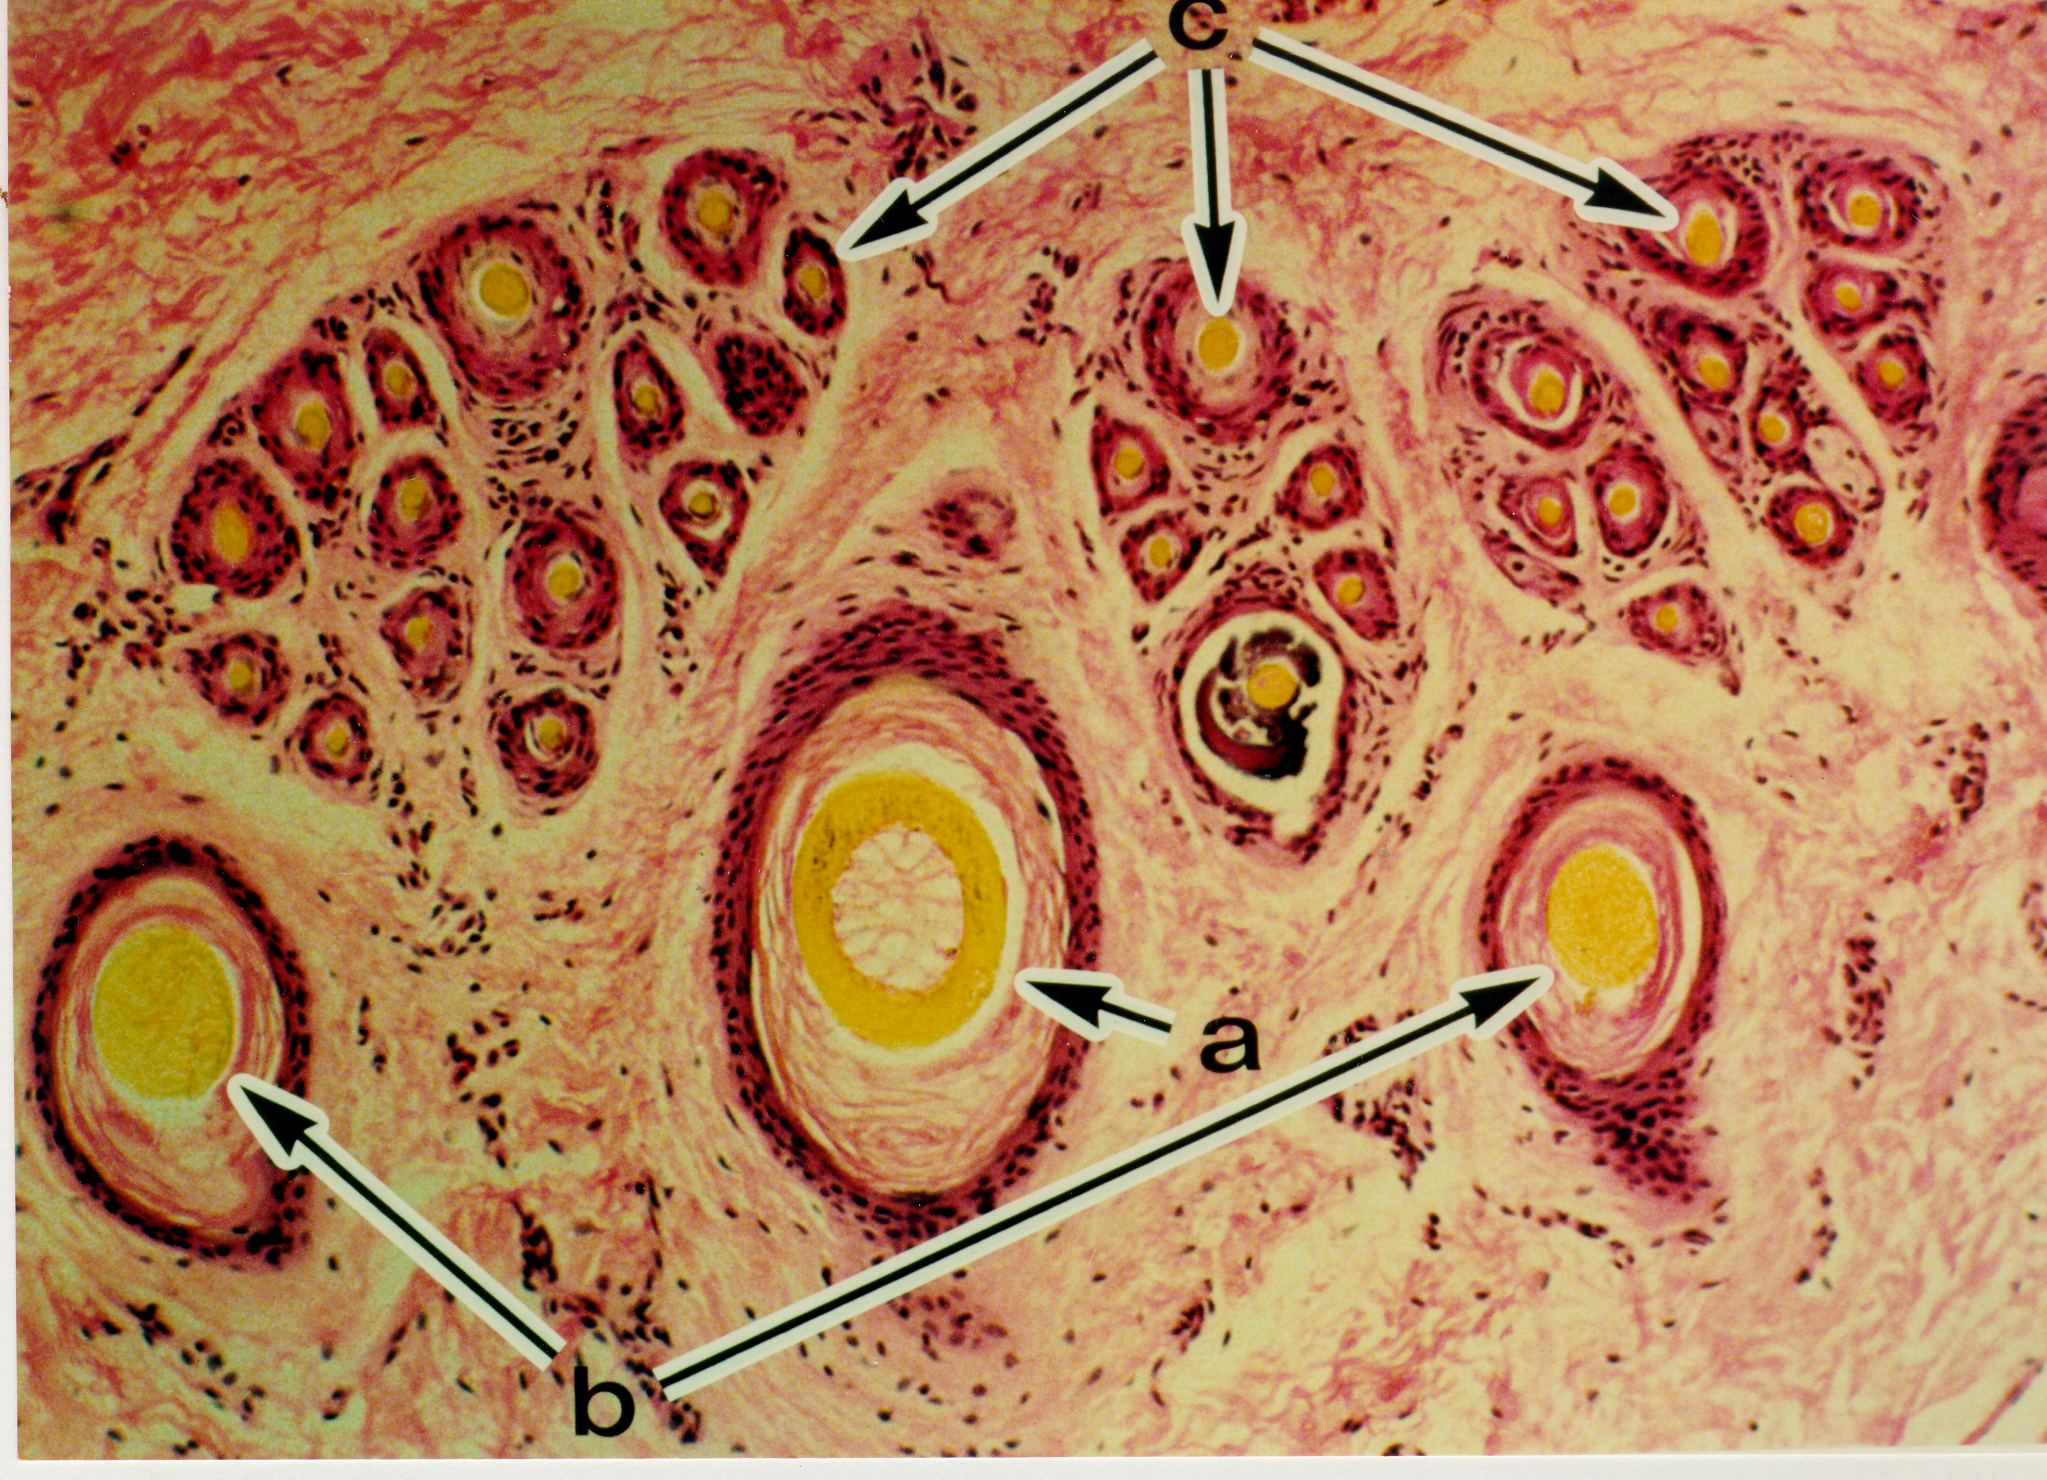
\includegraphics[width=\textwidth, trim = 0 20 0 120]{images/fig1a.png}
  }
  \subfigure[Plate (ii) x... magnification.]{
    \label{fig:1(ii)}
    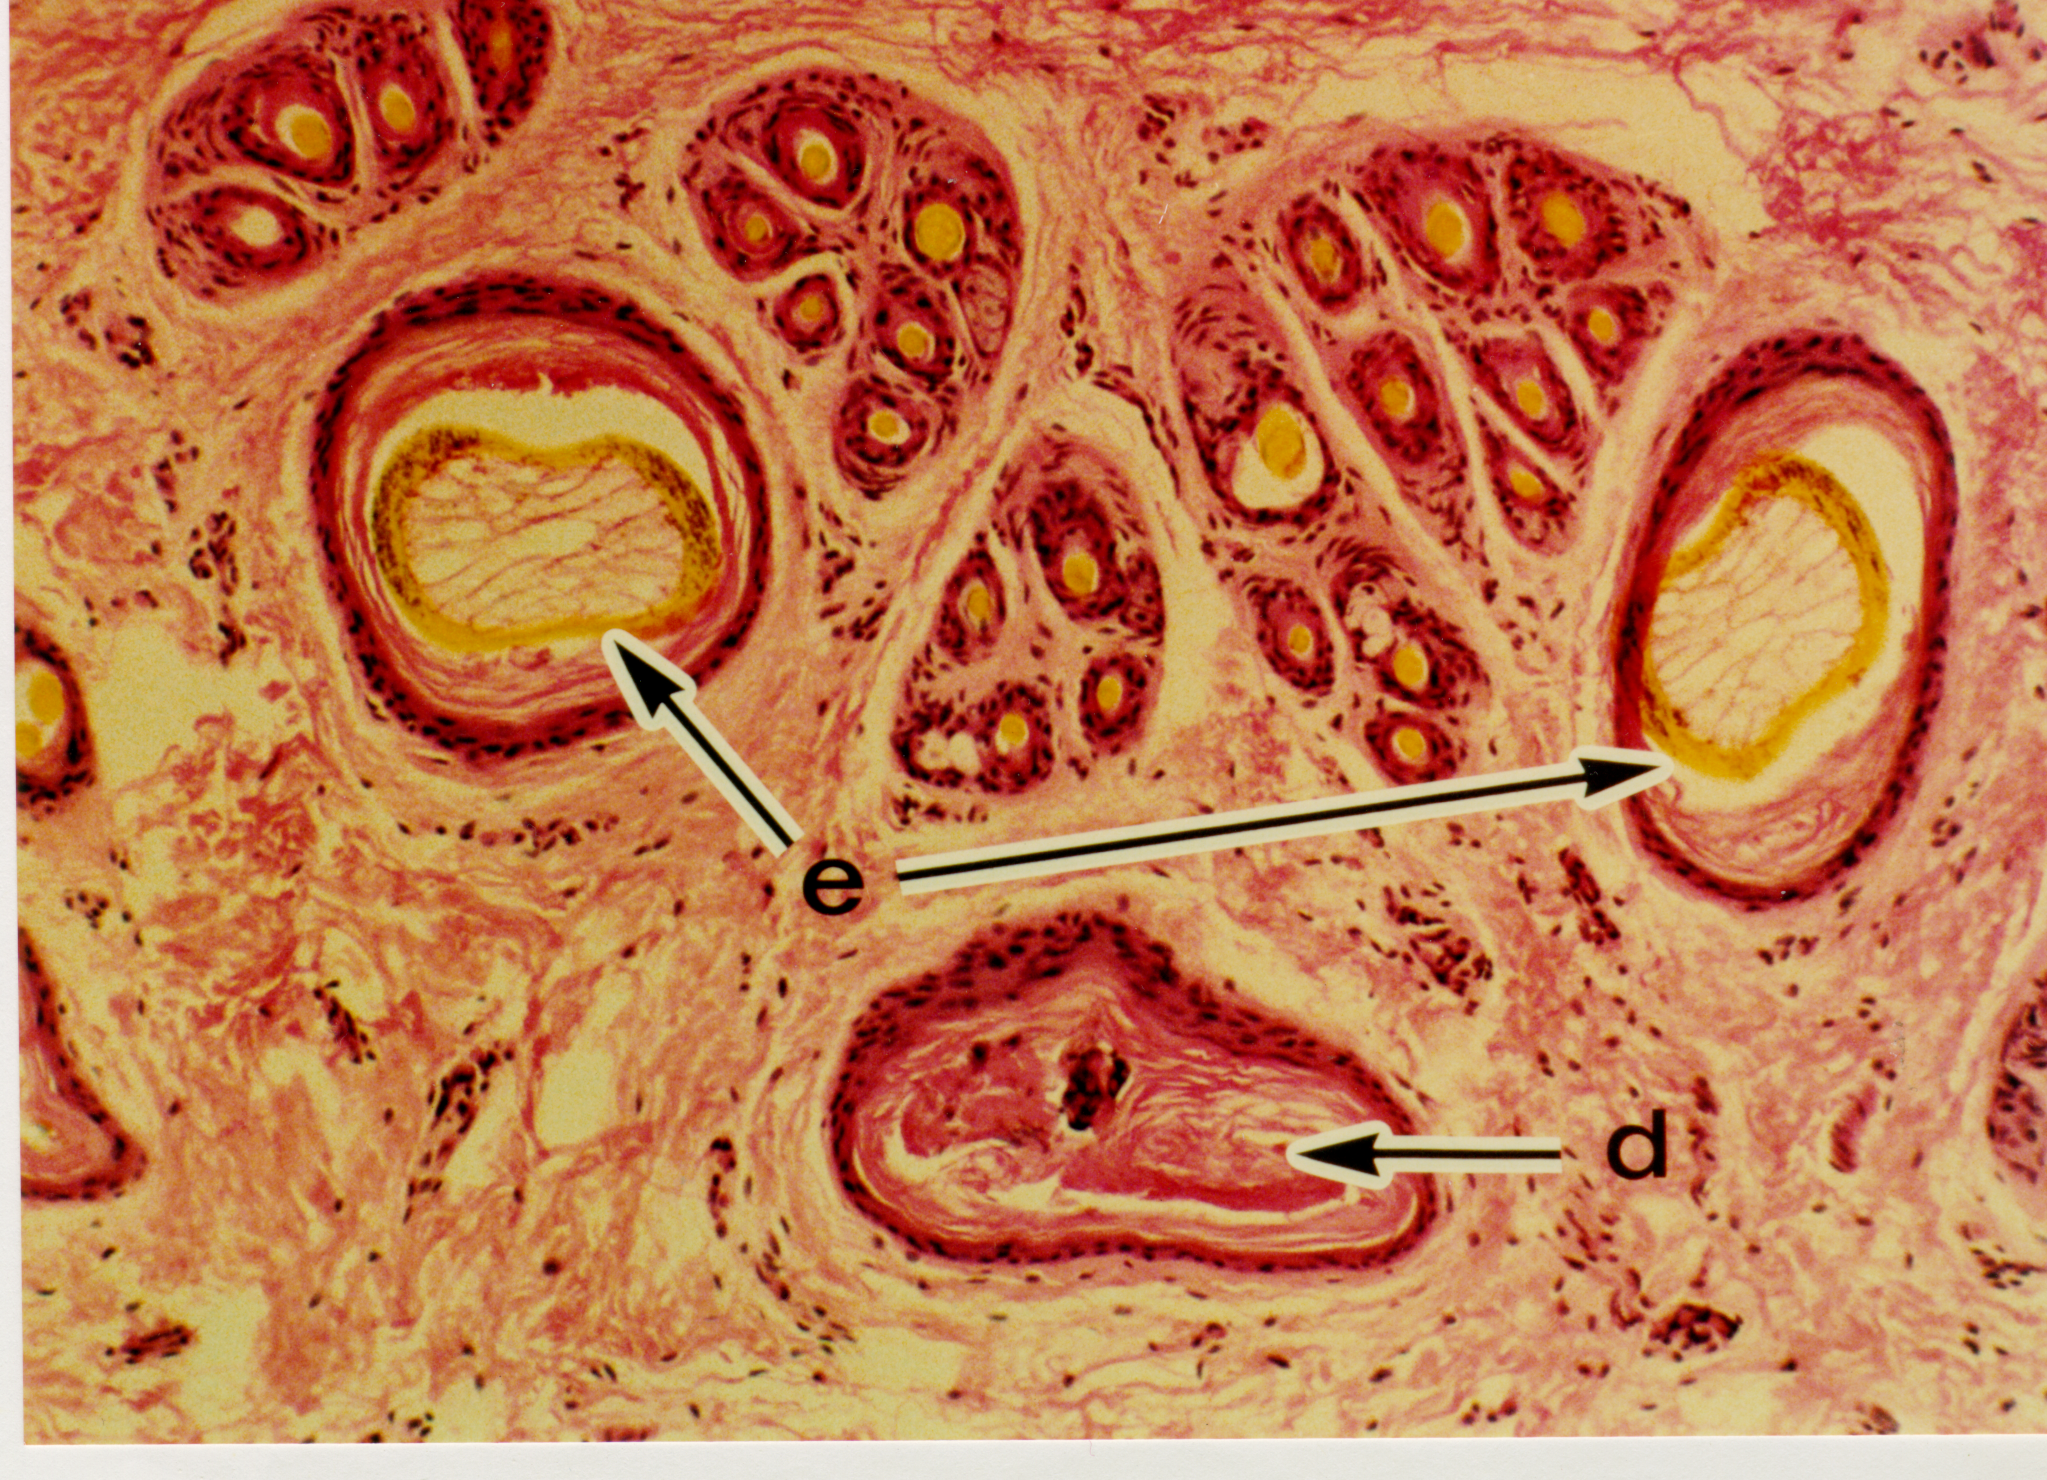
\includegraphics[width=\textwidth, trim = 0 20 0 20]{images/fig1b.png}
  }
  \caption{Transverse sections of skin from a primitive Barbary sheep
      showing (a) medullated central primary fibre ($150 \mu m$), (b)
      large primary lateral fibres ($80 \mu m$), (c) groups of fine
      secondary fibres ($15 \mu m$), (d) primary central follicle which
      has shed its fibre showing collapsed follicle wall, (e)
      medullated primary lateral fibres ($100 \mu m$).  The follicle
      groups have an average of nine secondaries per primary and the
      `wedge shaped' arrangement of secondaries is a consistent
      feature. }
  \label{fig:1}
\end{figure}

%\end{document}
